\chapter{Simile}
\label{chap:simile}
In this chapter we present our approach that seizes Continuous Integration process in order to recommend similar components that are being developed in a software project. The idea of integrating CI and Software reuse emerged with the following research question: \emph{How can code search engines be best married with CI?}. The idea was to find a way where a team could seize the continuous integration process in order to find similar components to the components they are developing. Thus they would be able to reuse instead of implementing them from scratch reducing development time and costs. As an attempt to answer the question we implemented a tool (proof of concept) called Simile. This tool analyses the source code and extract information needed to find similar components.

Following the usage scenario explained previously in section \ref{usage-scenario}, we will describe how our proposed approach works:

\begin{figure}[H]
	\centering
    \includegraphics[width=0.8\textwidth]{grafiken/simile-approach}
    \caption{Simile approach}
    \label{fig:simile-01}
\end{figure}

In the first step (figure \ref{fig:simile-01} - 1) the developer commits code to its local VCS. Then when the developer decides to push changes to the remote repository, the CI server is triggered (figure \ref{fig:simile-01} - 2). In the next step (figure \ref{fig:simile-01} - 3), Simile will analyse the code and extract information such as interfaces signatures and test classes. This information will be sent to SOCORA (figure \ref{fig:simile-01} - 4) in order to find similar components. Then it will return a ranked list of similar components. Simile will receive this information and send this list to the developers by email (figure \ref{fig:simile-01} - 5).

The main objective of Simile is to help the team to find similar components so they would be able to reuse them. Thus they would reduce time development and costs through reuse components that are already tested and ready to work.

In the following sections we will explain in details how Simile was implemented. Then we will detail how we integrate Simile into Continuous Integration server (Jenkins). After that we will explain how we integrate Simile and SOCORA for searching for similar components.

\section{Design}
Simile was formulated as a microservice which was designed taking in account that there are several CI servers available. Although we used Jenkins as CI server for our prototype, Simile was designed as an agnostic tool. Figure \ref{fig:simile-design} depicts an overview of the design of our implementation.

\begin{figure}[H]
	\centering
    \includegraphics[width=0.9\textwidth]{grafiken/simile-design}
    \caption{Overview of implementation's design}
    \label{fig:simile-design}
\end{figure}

Despite the fact that the design is rather simple, this allow us to connect Simile to any CI server available in the market without changing the core. For instance, if in the future we would like to support another CI servers such as Teamcity, TravisCI, or Buddy, we would just need to develop a simple plugin with the same features of the current plugin developed for this thesis. Figure \ref{fig:simile-future} depicts the hypothetical scenario described before.

\begin{figure}[H]
	\centering
    \includegraphics[width=0.9\textwidth]{grafiken/simile-future}
    \caption{Future scenario of Simile supporting several CI Servers}
    \label{fig:simile-future}
\end{figure}

Figure \ref{fig:domain-model} represents the domain model of Simile. The main class is \emph{Simile}, which is a service in charge of starting the process of analyzing the code, make request to SOCORA, and send the email to recipient with the candidates. This class instantiates a \emph{Cloner} and a \emph{DirectoryExplorer} in the method \emph{searchForComponent}. The former class is in charge of cloning the project to be analyzed and the latter is in charge of analyzing the code of the cloned project. Then the service \emph{SocoraRequester} is in charge of taking the information generated by \emph{DirectoryExplorer} and make the request to SOCORA to search for components. This service, after getting the result from SOCORA, it sends an email with the candidates (represented by the class \emph{Candidate}) to the recipient. 

\begin{figure}[H]
	\centering
    \includegraphics[width=\textwidth]{grafiken/domain-model}
    \caption{Domain model}
    \label{fig:domain-model}
\end{figure}

\section{Implementation}
In this section we will detail how the prototype was developed and the technologies used. First we will start explaining the Simile service which is the starting point of the whole process about cloning the project, analyse code, search components and send result. Then we will continue with the  HTTP controller which receives the Git repository of the project to be analysed, the specific branch of the repository, and the email where the result will be sent. Then we will explain the Cloner object which is in charge of cloning the project locally. After that, we will explain how the tool analyses the code and extracts the interface signatures and test classes which will be used to make the requests to SOCORA. Next we will describe how we receive the result from SOCORA. Finally we will explain how we handle the result from the previous step and build the email that will be sent to user.

\textbf{NOTE: The code snippet shown in the following subsections has been cleaned and it does not represent the source code. To see the source code with all the details, please refer to the appendix \ref{append:simile-code} or to the CD attached to this work.}

\subsection{Simile}
The class Simile.java [\ref{Simile.java}] is a Spring service which contains only one method, \emph{searchForComponents}. This methods receives four parameters, repo, branch, folder, and recipient. \emph{repo} represents the Git repository of the project to be analysed. \emph{branch} is the branch of the Git repository (optional). \emph{folder} represents the name of the folder where the project will be cloned. Finally \emph{recipient} is the email where Simile will send the result. Listing \ref{searchForComponents} represents the method.

\lstinputlisting[
  language=Java, numbers=left, firstnumber=1, breaklines=true, 
  basicstyle=\footnotesize,
  numberstyle=\tiny,
  caption={Method searchForComponents of Simile.java},
  captionpos=b,
  label=searchForComponents
]
{code/Simile-searchForComponents.txt}

First, it clones the project in the server by calling the method \emph{cloneRepository} of Cloner [\ref{Cloner.java}]. Then it analyses the Java main code of the project cloned and the test classes. When it analyses the code it extracts the interface signatures and the test classes, we explain how it does this process in section \ref{code-analysis}. With the result of the previous step, we make the requests to SOCORA to search for similar components.

It is important to notice that this method is asynchronous by the Java annotation \emph{@Async}. This allows us to run this method many times in parallel (configured in SimileApplication.java \ref{SimileApplication.java}).

\subsection{Cloner}
\label{simile:cloner}
The class Cloner.java [\ref{Cloner.java}] is in charged of cloning the project in a local directory. The listing \ref{cloneRepository} represents the method \emph{cloneRepository}.

\lstinputlisting[
  language=Java, numbers=left, firstnumber=1, breaklines=true, 
  basicstyle=\footnotesize,
  numberstyle=\tiny,
  caption={Method cloneRepository of Cloner.java},
  captionpos=b,
  label=cloneRepository
]
{code/Cloner-cloneRepository.txt}

This method runs the command \emph{git clone} with the parameters \emph{repo}, \emph{branch}, and \emph{folder}. The command is built by the private method \emph{setCommand}. After running the command, the project is cloned locally under the folder with given \emph{folder} name.

\subsection{Interface signature and test class extraction}
\label{simile:code-analysis}
In this section we will explain how Simile explores the project cloned and extracts the interface signatures and test classes that will be sent to SOCORA to search for similar components.

After the project is cloned locally by the Cloner (\ref{simile:cloner}), Simile goes through the code and extract interface signatures of each class, and test classes. The signatures extracted are transformed into Merobase Query Language (MQL) notation, and the test classes are extracted as is. The snipped code \ref{handler} shows how the interface signatures are extracted and transformed into MQL. For extracting test classes the principle is the same, the difference is that we differentiate a Test class from another Java file if it contains the annotation \emph{@Test}.

\lstinputlisting[
  language=Java, numbers=left, firstnumber=1, breaklines=true, 
  basicstyle=\footnotesize,
  numberstyle=\tiny,
  caption={Method handle of JavaClassHandler.java},
  captionpos=b,
  label=handler
]
{code/JavaClassHandler-handle.txt}

In the class JavaClassVisitor.java we can see how Simile differentiate between a normal Java class and a test class. It implements the methods \emph{visit} for a \emph{ClassOrInterfaceDeclaration} and for a \emph{MethodDeclaration} object of the abstract class VoidVisitorAdapter. The listing \ref{visit} show the implementation of these methods.

\lstinputlisting[
  language=Java, numbers=left, firstnumber=1, breaklines=true, 
  basicstyle=\footnotesize,
  numberstyle=\tiny,
  caption={Implementation of methods \emph{visit} of VoidVisitorAdapter in JavaClassVisitor.java},
  captionpos=b,
  label=visit
]
{code/JavaClassVisitor-visit.txt}

\subsection{SOCORA Integration}
\label{socora-integration}
Our prototype uses SOCORA to search for components. After extracting the interface signatures and test classes from the project, Simile make requests to SOCORA using this information. SOCORA then searches for similar components using Merobase and ranks the candidates using non-functional requirements. Once it is done, SOCORA sends the result back to Simile.

Simile communicates with SOCORA by making HTTP requests using the interface signatures and the test classes extracted. The following snippet of code show how Simile is making the request for SOCORA \ref{textualSearchComponent}.

\lstinputlisting[
  language=Java, numbers=left, firstnumber=1, breaklines=true, 
  basicstyle=\footnotesize,
  numberstyle=\tiny,
  caption={Method textualSearchComponent of SocoraRequester.java},
  captionpos=b,
  label=textualSearchComponent
]
{code/SocoraRequester-textualSearchComponent.txt}

The class in charge of making the request to SOCORA is \emph{SocoraRequester.java}[\ref{SocoraRequester.java}]. The method \emph{searchComponent} receives two parameters, \emph{queries} which represents the interface signatures or the test classes, and \emph{searchType} which represents the type of search (i.e. test driven search, interface driven search or textual search (default)). The snippet of code \ref{searchComponent} represent the method \emph{searchComponent}.

\lstinputlisting[
  language=Java, numbers=left, firstnumber=1, breaklines=true, 
  basicstyle=\footnotesize,
  numberstyle=\tiny,
  caption={Method searchComponent of SocoraRequester.java},
  captionpos=b,
  label=searchComponent
]
{code/SocoraRequester-searchComponent.txt}

When SOCORA responses with the list of components found they are sent by email to developers. This action is done in the methods \emph{textualSearchComponent} or \emph{testDrivenSearchComponent} using the service EmailSender [\ref{EmailSender.java}].

\subsection{Email result}
After making the requests to SOCORA \ref{socora-integration}, it will response with the candidate components found. Simile receives the list of candidates, it extracts the candidates from the response, builds the email, and sends it to the recipient. For textual search results, the method \emph{processTemplateTextualSearchResult} is in charge of interpreting the result and process the email's template before it is sent. For test-driven results, the method \emph{processTemplateTestDrivenSearchResult} is in charge of interpreting the result and process the email's template before it is sent. The listing \ref{resultInterpretation} show this method.

\lstinputlisting[
  language=Java, numbers=left, firstnumber=1, breaklines=true, 
  basicstyle=\footnotesize,
  numberstyle=\tiny,
  caption={Methods \emph{processTemplateTextualSearchResult} and \emph{processTemplateTestDrivenSearchResult} of SocoraRequester.java},
  captionpos=b,
  label=resultInterpretation
]
{code/SocoraRequester-responseInterpretation.txt}

After the email's body is generated by using the template and the java objects, it is sent to the recipient. The figures \ref{fig:email-01} and \ref{fig:email-02} show the email with the result of a textual search and a test-driven search respectively.

\begin{figure}[H]
	\centering
    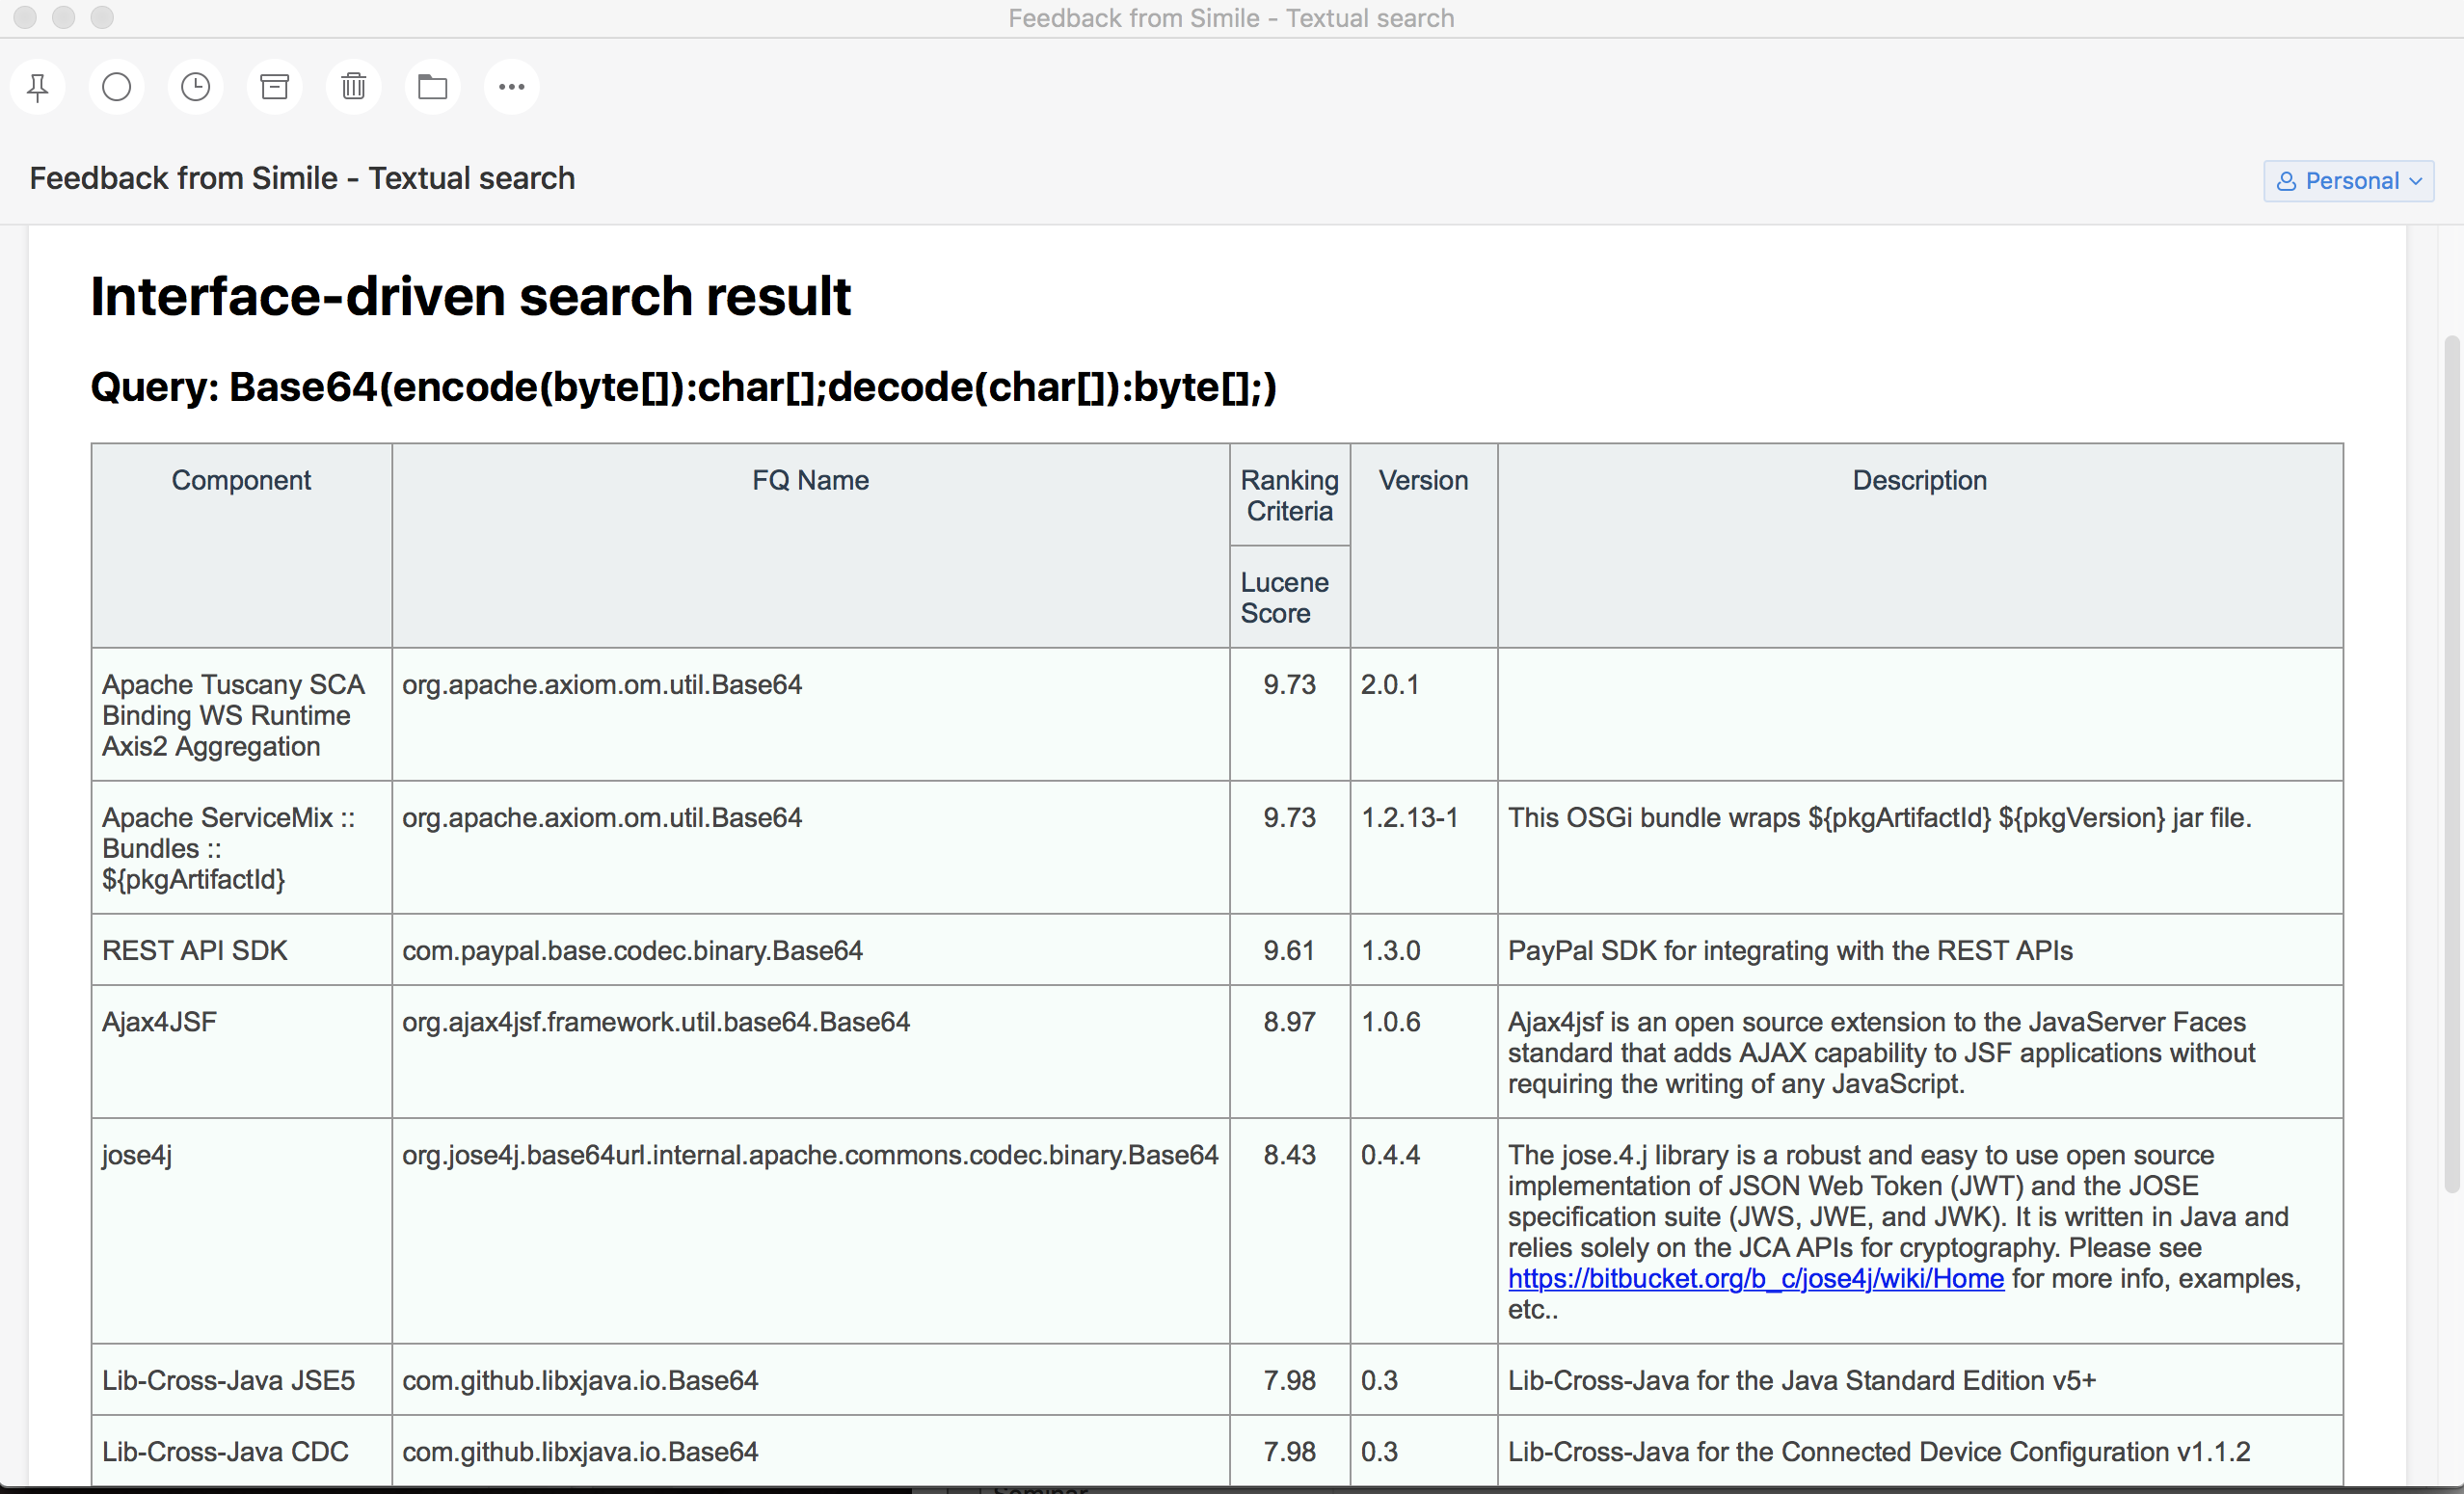
\includegraphics[width=0.8\textwidth]{grafiken/email-01}
    \caption{Textual search result email}
    \label{fig:email-01}
\end{figure}

\begin{figure}[H]
	\centering
    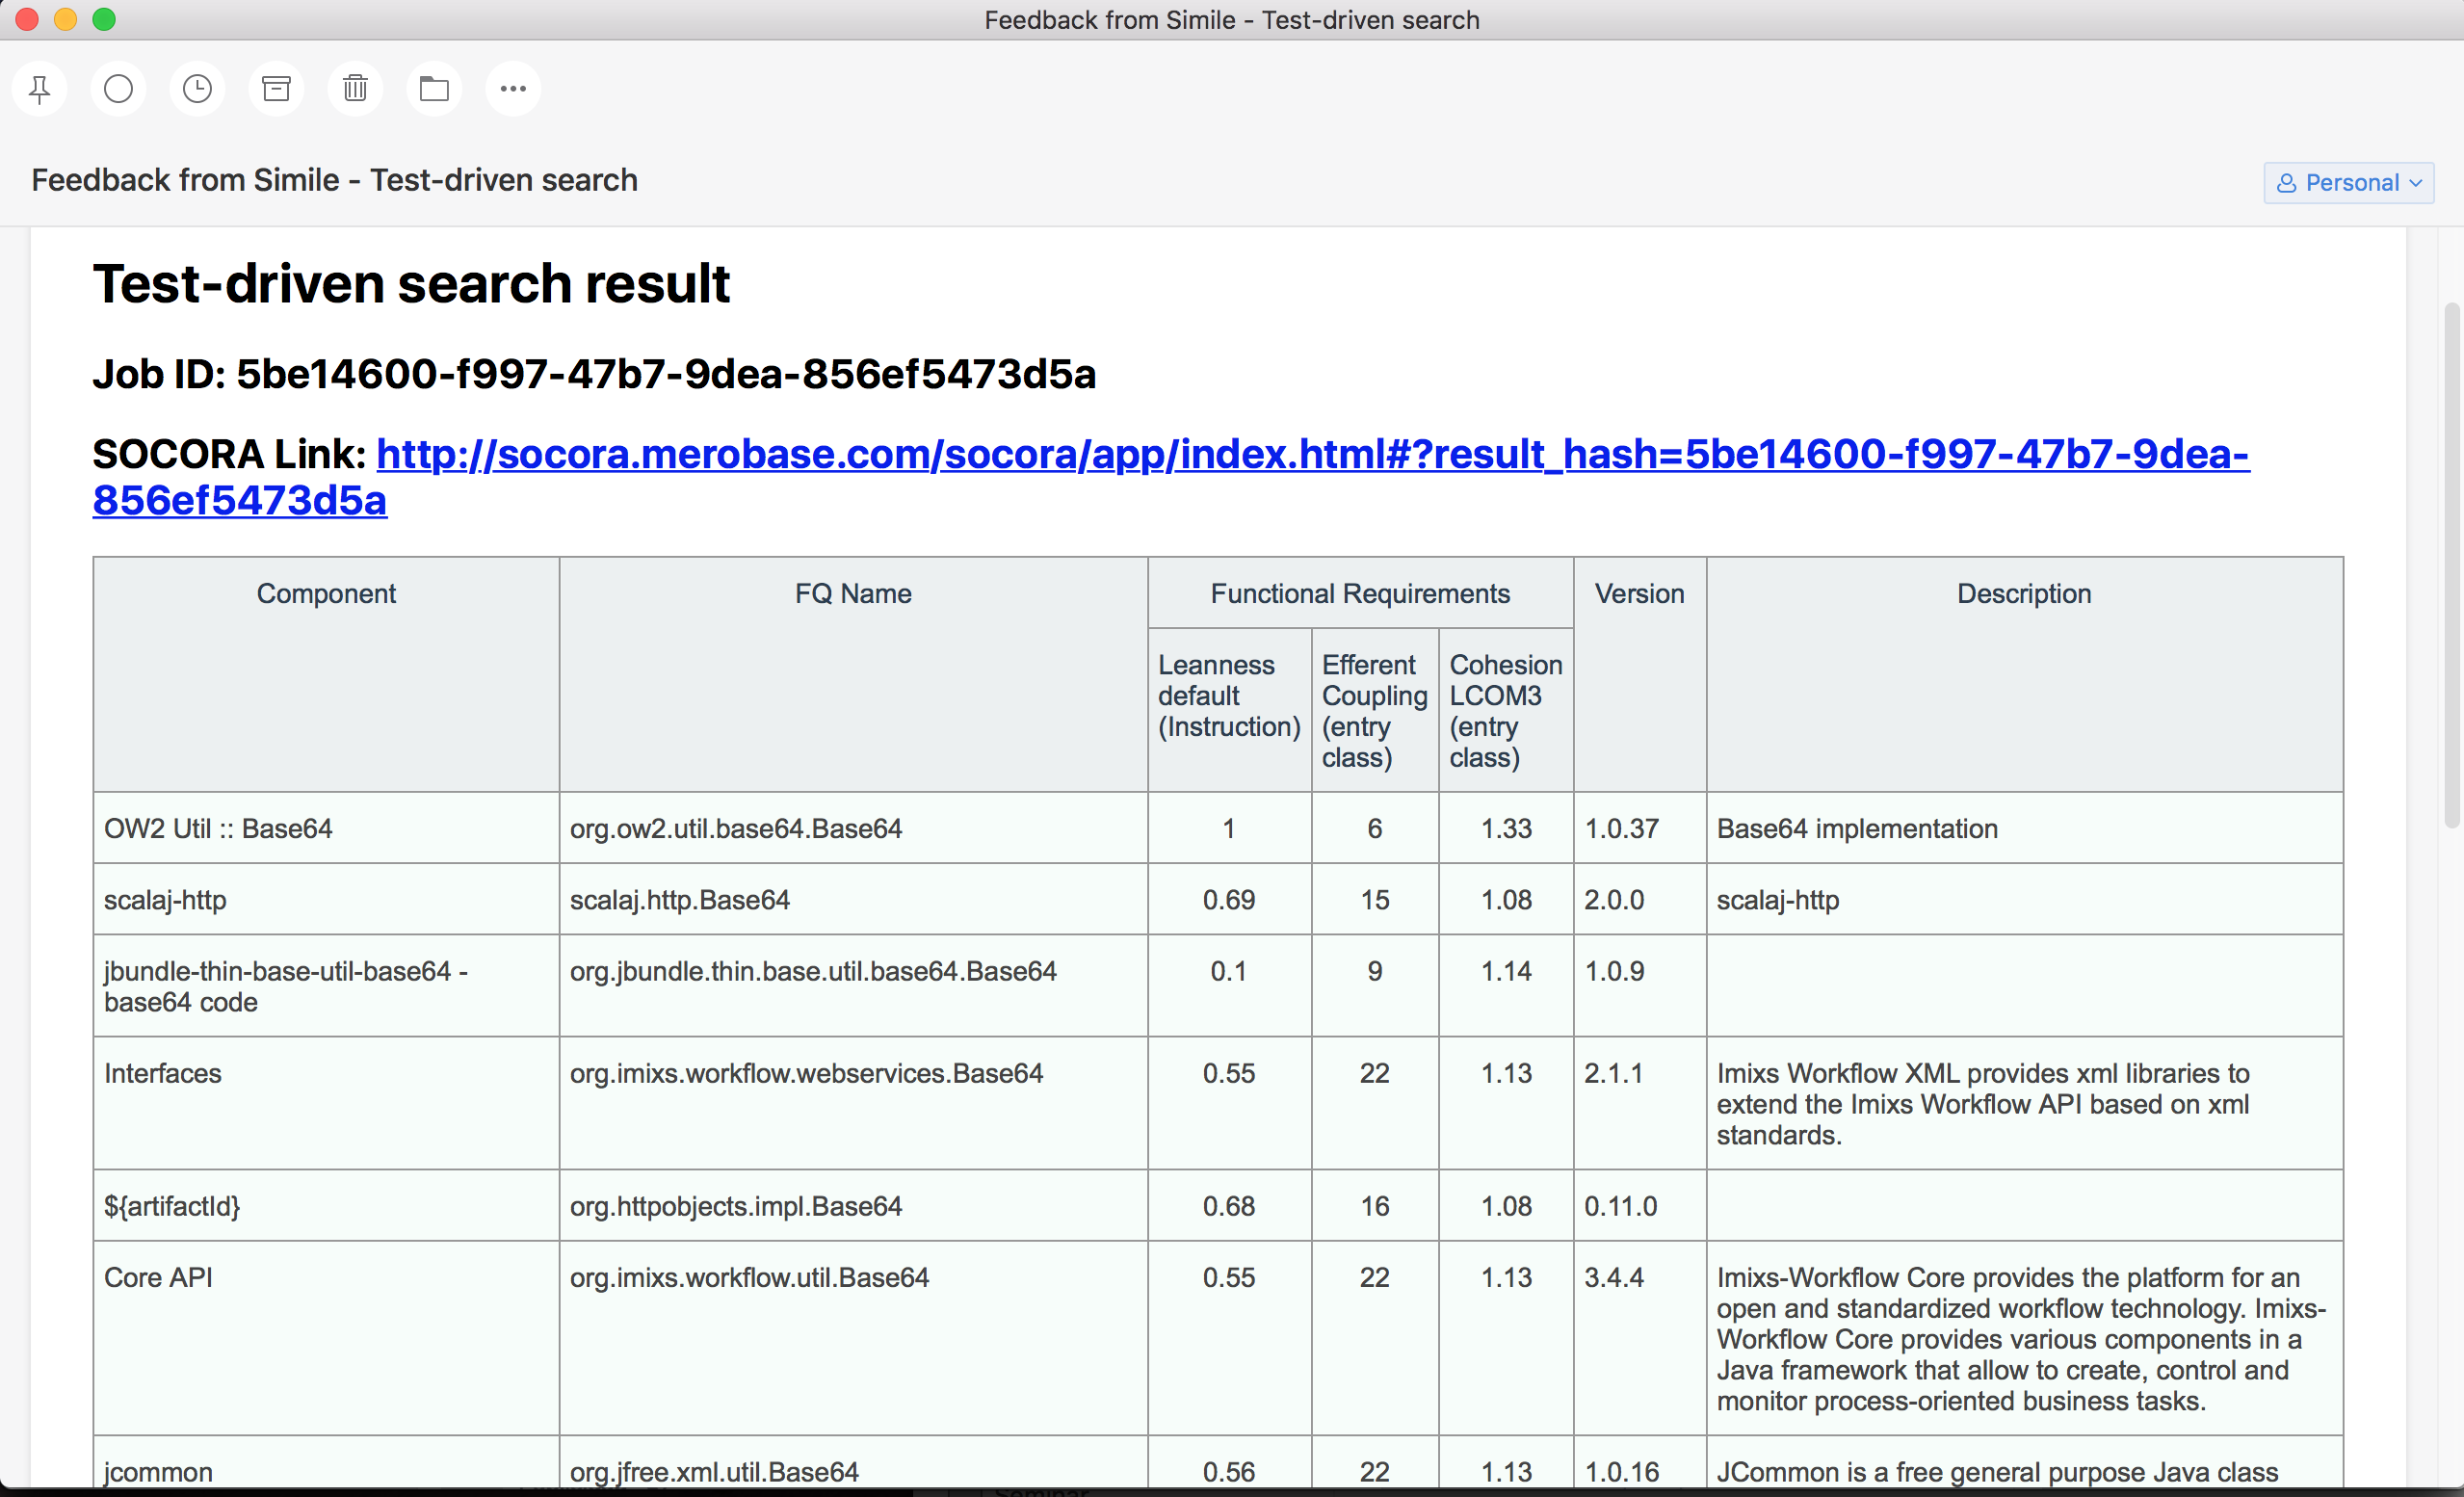
\includegraphics[width=0.8\textwidth]{grafiken/email-02}
    \caption{Test-driven search result email}
    \label{fig:email-02}
\end{figure}

Depending on the type of search, the email will have some differences. The text driven search result contains a the query sent to SOCORA and a table with the candidates found. For test-driven search result, the email contains the job id of the search, the link to SOCORA to see more details of the result and the list of candidates found.

\subsection{HTTP Controller}
The Java class EntryController.java [\ref{EntryController.java}] is in charge of receiving the request from a customer with the Git repository and the branch of the project to be analysed, and the email where the result of the similar component will be sent. In the listing \ref{setupRepository} we can see the method \emph{setupRepository} which represents the entry point which is a POST request with the three parameters described before. The parameter \emph{repo} is required and represent the Git repository of the project that will be analysed and to which similar components will be searched for. The parameter \emph{branch} represents the branch of the git repository, this parameter is optional. Finally, the parameter \emph{email} represents the email where the result of the similar components will be sent to.

\lstinputlisting[
  language=Java, numbers=left, firstnumber=1, breaklines=true, 
  basicstyle=\footnotesize,
  numberstyle=\tiny,
  caption={Method setupRepository of EntryController.java},
  captionpos=b,
  label=setupRepository
]
{code/EntryController-setupRepository.txt}

When a request is received by the controller, it firstly validates if the parameters are correct. If they are not valid, it will respond with HTTP status code 400 and a message describing the errors. Otherwise, it triggers asynchronously the method searchForComponents with the repository, the branch, and a random CUID as a folder name of the service Simile. This service is in charge of starting the process of cloning the project, analyse the code, make the request to SOCORA, and to send the email with the result to the customer.

\section{CI integration}
\label{ci-integration}
To integrate our prototype to a Continuous Integration process we decided to create a plugin. We decided to create our main prototype as independent as possible thus we do not depend on any CI tool. Therefore in this work to prove our approach we built a plugin for the CI server Jenkins. We decided to use Jenkins because is one of the most popular CI server for Java projects \footnote{\url{https://www.cloudbees.com/sites/default/files/2016-jenkins-community-survey-responses.pdf} (accessed: 04.02.2017)} and it is open-source.

The Simile Jenkins plugin is simple. First when a user creates a job in Jenkins, he/she can add a post build step. There he/she select the Simile plugin. When it is done, a new section is added in the task configuration (figure \ref{fig:simile-conf-01}). There he/she should add the Git repository of the project, the branch (optional), and the email. Once done, whenever the job is triggered, the plugin will be triggered too. The plugin sends via HTTP POST request the repository, branch, and email to Simile.

\begin{figure}[H]
	\centering
    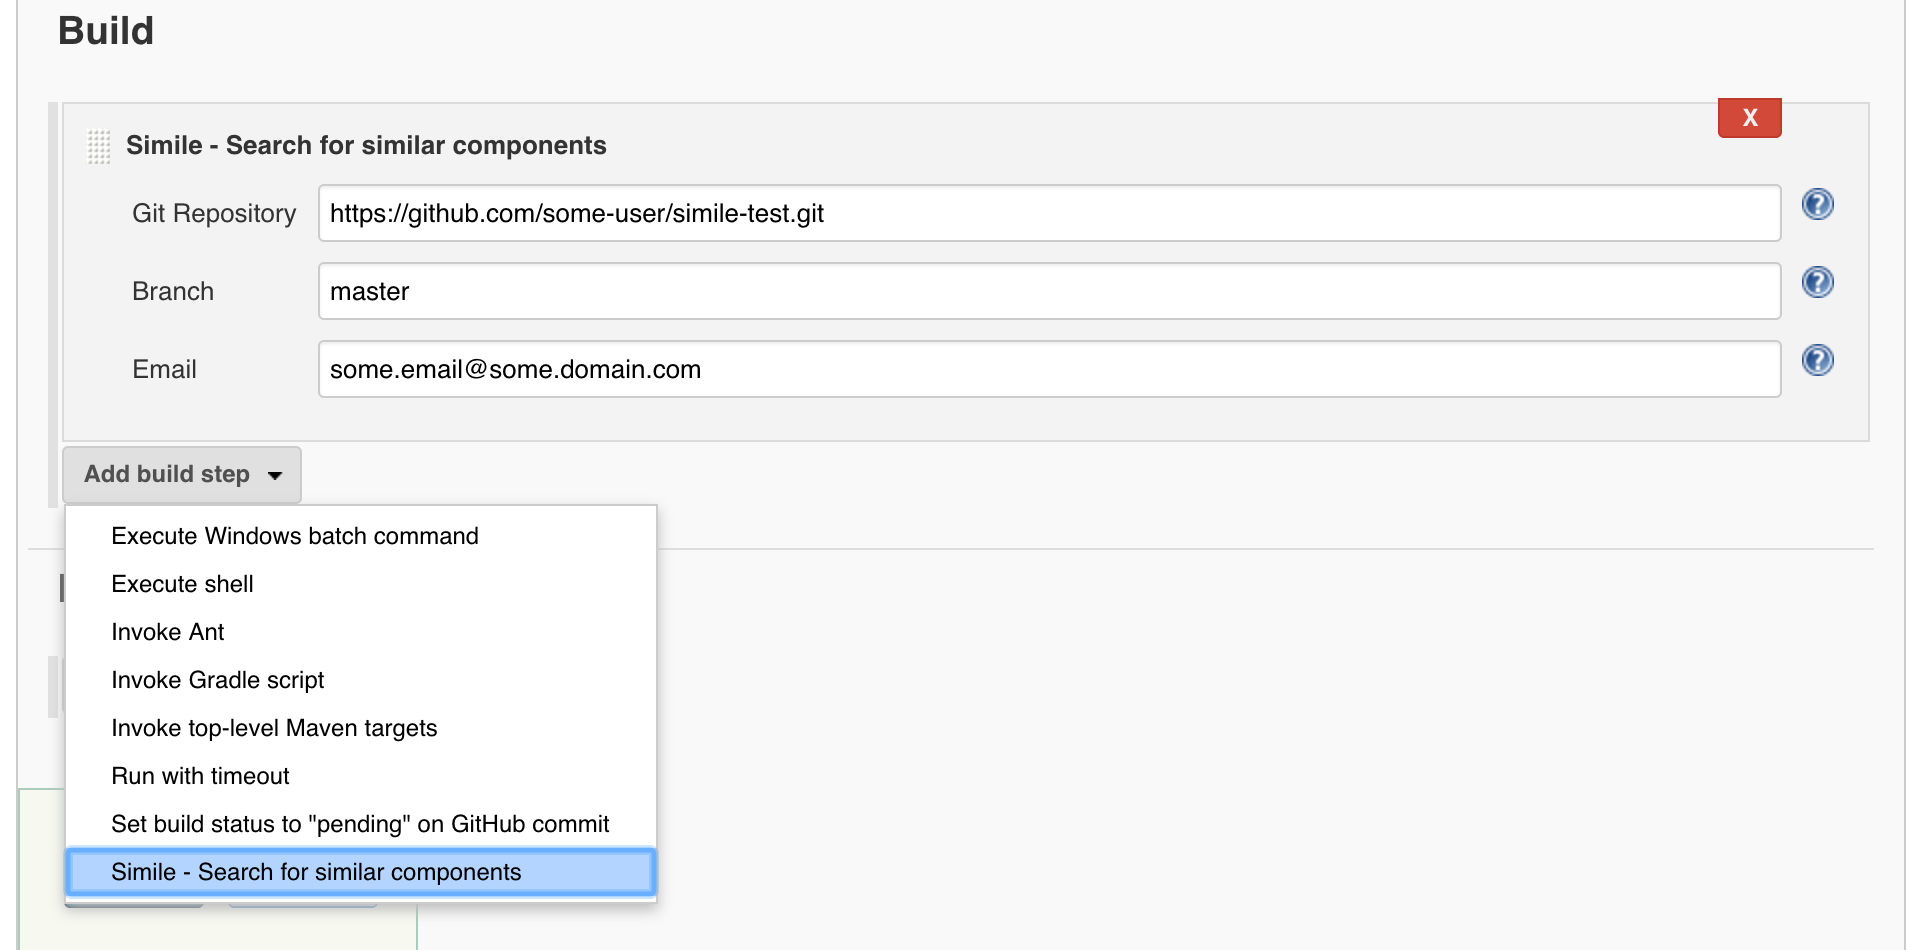
\includegraphics[width=0.9\textwidth]{grafiken/simile-conf-01}
    \caption{Simile Jenkins plugin configuration in Jenkins task}
    \label{fig:simile-conf-01}
\end{figure}

To configure the endpoint where Simile is deployed, we just need to go to global settings and set the URL. Figure \ref{fig:simile-conf-02} depicts this option.

\begin{figure}[H]
	\centering
    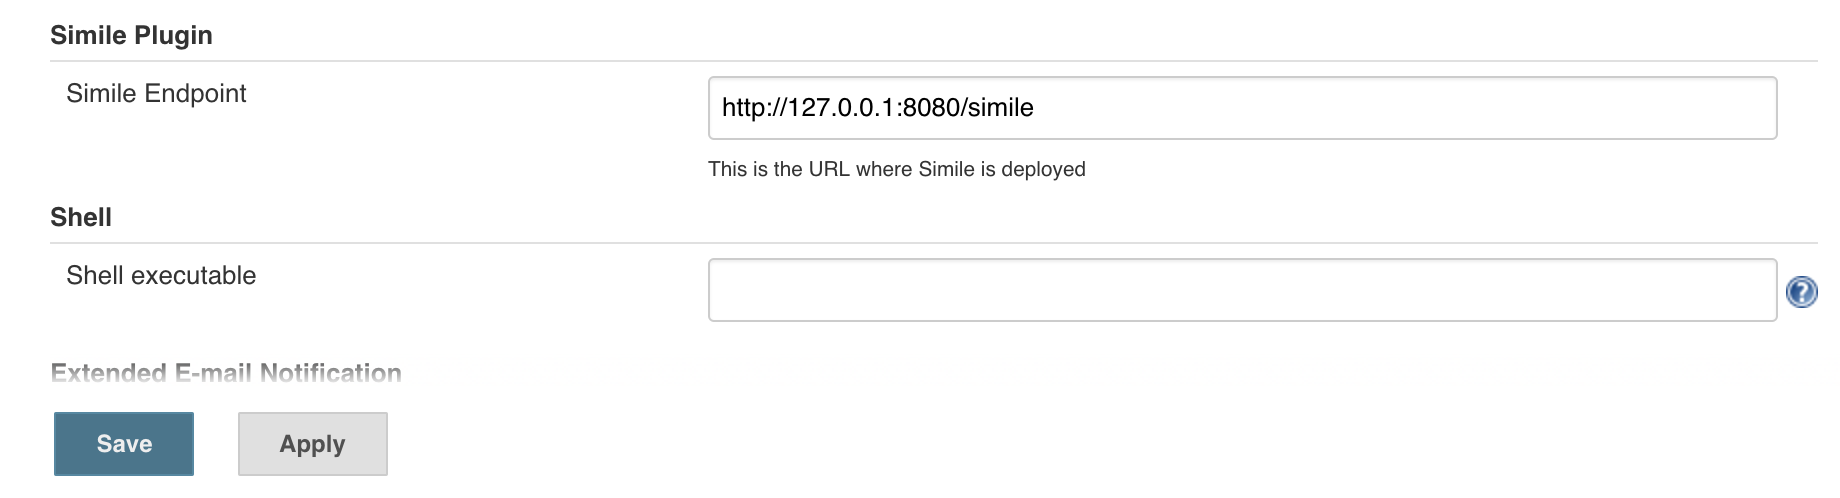
\includegraphics[width=0.9\textwidth]{grafiken/simile-conf-02}
    \caption{Simile endpoint configuration in Jenkins global configuration}
    \label{fig:simile-conf-02}
\end{figure}

In the future if Simile needs to be integrated to another CI server, we just need to develop a simple plugin which sends the information needed to look for similar components.

As a conclusion in Figure \ref{fig:sequence-diagram} we can appreciate how the objects interact with each other. The process begins with the method \emph{searchRepository} which contains the repository of the project, the branch and the email where the result will be sent. It triggers the method \emph{searchForComponent} of the service Simile asynchronously. Right after the project is cloned locally by Cloner object and it is explored by DirectoryExplorer object. After the classes, its methods, and test classes are extracted from the project, we get into two loops. In the first loop, for each Java class extracted Simile makes a request to SOCORA. The query is the class extracted defined in MQL notation. Once the result set is returned by SOCORA, Simile prepares the email with the candidates and sends them to the recipient.
 
\begin{figure}[H]
	\centering
    \includegraphics[width=\textwidth]{grafiken/sequence-diagram}
    \caption{Sequence diagram}
    \label{fig:sequence-diagram}
\end{figure}

\section{Search Results}
In this section we will evaluate the results obtain using Simile in our test-project. To test our proof-of-concept we used a project that implements the usage scenario we explain in Chapter \ref{usage-scenario}. First, we deployed Jenkins in a Tomcat 9 instance and we installed the Simile Jenkins Plugin. After that we created a task in Jenkins and we configured the plugin following the steps described in Section \ref{ci-integration}. Then we ran the task to get the candidates for component reuse. Finally we received the result and measured the number of candidates returned by SOCORA, non-functional requirements, and time taken to return the results.

\subsection{Textual search}
For textual search, Simile takes the classes and the method it contains, and then transform them into MQL notation. Our test project has only one class \emph{Base64.java} (Listing \ref{Base64.java}, page \pageref{Base64.java}) which contains two methods: \emph{encode} and \emph{decode}. The MQL notation of this class is the following:

\begin{displayquote}
\emph{Base64(encode(byte[]):char[];decode(char[]):byte[];)}
\end{displayquote}

By default the application used the following query parameters:

\begin{itemize}
\item Filters
	\begin{itemize}
	\item Entry class hashcode clone\footnote{Filters out additional entry class hash clones}
	\item No abstract class\footnote{Filters out abstract classes}
	\item No interface\footnote{Filters out interfaces}
	\item Latest version\footnote{Filters Maven-based components based on later versions}
	\item Functional sufficiency
	\end{itemize}
\item Ranking Strategy
	\begin{itemize}
	\item Single objective
	\end{itemize}
\item Ranking criteria
	\begin{itemize}
	\item Lucene score - objective: maximize
	\end{itemize}
\item Others
	\begin{itemize}
	\item Max number of results = 10
	\end{itemize}
\end{itemize}

Using the MQL notation of the class and the parameters, Simile makes the request to SOCORA. The code can be found in class \emph{SocoraRequester.java} in method \emph{textualSearchComponent} (Listing \ref{SocoraRequester.java}, page \pageref{SocoraRequester.java}). 

Table \ref{textual-result} details the result returned by SOCORA. The candidates are sorted by Lucene score, the higher the number more similar is the result to the query. Therefore the first candidate, org.apache.axiom.om.util.Base64\footnote{\url{http://grepcode.com/file/repo1.maven.org/maven2/org.apache.ws.commons.axiom/axiom-api/1.2.15/org/apache/axiom/util/base64/Base64Utils.java} (accessed: 21.02.2017)}, is more similar to the query than the last candidate, org.jboss.as.process.stdin.Base64\footnote{\url{https://github.com/wildfly/wildfly-core/blob/master/process-controller/src/main/java/org/jboss/as/process/stdin/Base64.java} (accessed: 21.02.2017)}. If we check the code of these candidates, we can see that the first one actually implements the two methods of the query using the same input but with different output. Whereas the last one implements the methods but with different inputs and outputs.

\begin{table}[]
\centering
\resizebox{\textwidth}{!}{%
\begin{tabular}{|l|l|cll|c|}
\hline
\multicolumn{1}{|c|}{\multirow{2}{*}{Component}}                                                      & \multicolumn{1}{c|}{\multirow{2}{*}{FQ Name}}                    & \multicolumn{3}{c|}{\begin{tabular}[c]{@{}c@{}}Ranking \\ Criteria\end{tabular}} & \multirow{2}{*}{Version} \\ \cline{3-5}
\multicolumn{1}{|c|}{}                                                                                & \multicolumn{1}{c|}{}                                            & \multicolumn{3}{c}{\begin{tabular}[c]{@{}c@{}}Lucene\\ Score\end{tabular}}       &                          \\ \hline
\begin{tabular}[c]{@{}l@{}}Apache Tuscany SCA \\ Binding WS Runtime \\ Axis2 Aggregation\end{tabular} & org.apache.axiom.om.util.Base64                                  & \multicolumn{3}{c|}{9.73}                                                        & 2.0.1                    \\ \hline
\begin{tabular}[c]{@{}l@{}}Apache ServiceMix \\ Bundles\end{tabular}                                  & org.apache.axiom.om.util.Base64                                  & \multicolumn{3}{c|}{9.73}                                                        & 1.2.13-1                 \\ \hline
REST API SDK                                                                                          & com.paypal.base.codec.binary.Base64                              & \multicolumn{3}{c|}{9.61}                                                        & 1.3.0                    \\ \hline
Ajax4JSF                                                                                              & org.ajax4jsf.framework.util.base64.Base64                        & \multicolumn{3}{c|}{8.97}                                                        & 1.0.6                    \\ \hline
jose4j                                                                                                & org.jose4j.base64url.internal.apache.commons.codec.binary.Base64 & \multicolumn{3}{c|}{8.43}                                                        & 0.4.4                    \\ \hline
Lib-Cross-Java JSE5                                                                                   & com.github.libxjava.io.Base64                                    & \multicolumn{3}{c|}{7.98}                                                        & 0.3                      \\ \hline
Lib-Cross-Java CDC                                                                                    & com.github.libxjava.io.Base64                                    & \multicolumn{3}{c|}{7.98}                                                        & 0.3                      \\ \hline
Lib-Cross-Java CLDC                                                                                   & com.github.libxjava.io.Base64                                    & \multicolumn{3}{c|}{7.98}                                                        & 0.3                      \\ \hline
rfc-4648                                                                                              & com.googlecode.jinahya.rfc4648.Base64                            & \multicolumn{3}{c|}{7.96}                                                        & 1.0.2                    \\ \hline
WildFly: Process Controller                                                                           & org.jboss.as.process.stdin.Base64                                & \multicolumn{3}{c|}{7.64}                                                        & 8.2.1.Final              \\ \hline
\end{tabular}%
}
\caption{Textual search result}
\label{textual-result}
\end{table}

The time taken from making the request to SOCORA to receive the result was 6.07 seconds\footnote{This time does not consider the time taken to receive the email with the result.}.
\subsection{Test-driven search}
For test-driven search, Simile takes the test classes that the project might have. Our test project contains only one test class, \emph{Base64Test.java} (Listing \ref{Base64Test.java}, page \pageref{Base64Test.java}), which contains one test and two auxiliary methods. This test is taken by Simile as is and it is used as query.

By default the the query parameters for test-driven search are the following:

\begin{itemize}
\item Filters
	\begin{itemize}
	\item Entry class hashcode clone\footnote{Filters out additional entry class hash clones}
	\item No abstract class\footnote{Filters out abstract classes}
	\item No interface\footnote{Filters out interfaces}
	\item Latest version\footnote{Filters Maven-based components based on later versions}
	\item Functional sufficiency
	\end{itemize}
\item Ranking Strategy
	\begin{itemize}
	\item Hybrid non-dominated sorting
	\end{itemize}
\item Non-functional metrics
	\begin{itemize}
	\item Leanness default\footnote{Leanness based on instructions count (Needed Functionality/Necessary Functionality, [0, 1]. Default objective is to maximize} - objective: maximize
	\item Throughput operations per second - objective: maximize
	\item Cohesion LCOM3\footnote{LCOM3 cohesion (CK), scope entry class} - objective: minimize
	\item Efferent Coupling\footnote{Efferent Coupling of Entry Class (How many other classes are used by this class?)} - objective: minimize
	\end{itemize}
\item Others
	\begin{itemize}
	\item Max number of results = 400
	\end{itemize}
\end{itemize}

Using the test class and the query parameters, Simile makes the request to SOCORA. The code can be found in class \emph{SocoraRequester.java} in method \emph{testDrivenSearchComponent} (Listing \ref{SocoraRequester.java}, page \pageref{SocoraRequester.java}).

Table \ref{test-drive-result} details the result given by SOCORA for our test class with the query parameters. All of these candidates meet the functional requirements, so all of them might be reused. The difference is in the metrics. Neither the first component of the list is the best nor the last one is the worst, that is defined by the user's requirements. For this reason we include the link to the SOCORA webpage where the user can visualize this result and sort them based on its requirements. For instance, for one user might be more important the leanness value rather than the other, thus he/she would be more interested on the components with highest leanness value.

\begin{table}[]
\centering
\resizebox{\textwidth}{!}{%
\begin{tabular}{|l|l|c|c|c|c|}
\hline
\multicolumn{1}{|c|}{\multirow{2}{*}{Component}}                                                                & \multicolumn{1}{c|}{\multirow{2}{*}{FQ Name}} & \multicolumn{3}{c|}{Metrics}                                                                                                                                                        & \multirow{2}{*}{Version}                                     \\ \cline{3-5}
\multicolumn{1}{|c|}{}                                                                                          & \multicolumn{1}{c|}{}                         & \begin{tabular}[c]{@{}c@{}}Leanness\\ Default\end{tabular} & \begin{tabular}[c]{@{}c@{}}Efferent\\ Coupling\end{tabular} & \begin{tabular}[c]{@{}c@{}}Cohesion\\ LCOM3\end{tabular} &                                                              \\ \hline
OW2 Util :: Base64                                                                                              & org.ow2.util.base64.Base64                    & 1                                                          & 6                                                           & 1.33                                                     & 1.0.37                                                       \\ \hline
scalaj-http                                                                                                     & scalaj.http.Base64                            & 0.69                                                       & 15                                                          & 1.08                                                     & 2.0.0                                                        \\ \hline
Interfaces                                                                                                      & org.imixs.workflow.webservices.Base64         & 0.55                                                       & 22                                                          & 1.13                                                     & 2.1.1                                                        \\ \hline
jtstand-common                                                                                                  & org.jfree.xml.util.Base64                     & 0.56                                                       & 22                                                          & 1.13                                                     & 1.5.9                                                        \\ \hline
Macaroons: Cookies                                                                                              & com.github.nitram509.jmacaroons.util.Base64   & 0.95                                                       & 6                                                           & 1.13                                                     & 0.3.1                                                        \\ \hline
Core API                                                                                                        & org.imixs.workflow.util.Base64                & 0.55                                                       & 22                                                          & 1.13                                                     & 3.4.4                                                        \\ \hline
jcommon                                                                                                         & org.jfree.xml.util.Base64                     & 0.56                                                       & 22                                                          & 1.13                                                     & 1.0.16                                                       \\ \hline
TrAP Utils API                                                                                                  & com.ericsson.research.trap.utils.Base64       & 0.46                                                       & 16                                                          & 1.08                                                     & 1.4.1                                                        \\ \hline
\begin{tabular}[c]{@{}l@{}}jbundle-thin-base-util-\\ base64 - base64 code\end{tabular}                          & org.jbundle.thin.base.util.base64.Base64      & 0.1                                                        & 9                                                           & 1.14                                                     & 1.0.9                                                        \\ \hline
\begin{tabular}[c]{@{}l@{}}JASMINe :: Self \\ management :: Rules \\ :: Cluster :: JK \\ :: Common\end{tabular} & org.ow2.jasmine.rules.cluster.jk.Base64       & 1                                                          & 6                                                           & 1.33                                                     & 1.3.7                                                        \\ \hline
JPush API Java Client                                                                                           & cn.jpush.api.utils.Base64                     & 1                                                          & 5                                                           & 1.33                                                     & 3.2.7                                                        \\ \hline
Ganymed SSH2 for Java                                                                                           & com.trilead.ssh2.crypto.Base64                & 1                                                          & 5                                                           & 1.33                                                     & \begin{tabular}[c]{@{}c@{}}build212-\\ hudson-6\end{tabular} \\ \hline
ganymed-ssh-2                                                                                                   & ch.ethz.ssh2.crypto.Base64                    & 1                                                          & 5                                                           & 1.33                                                     & 262                                                          \\ \hline
\begin{tabular}[c]{@{}l@{}}Ganymed SSH2 \\ for Java\end{tabular}                                                & ch.ethz.ssh2.crypto.Base64                    & 1                                                          & 5                                                           & 1.33                                                     & \begin{tabular}[c]{@{}c@{}}build210-\\ hudson-1\end{tabular} \\ \hline
\begin{tabular}[c]{@{}l@{}}JOnAS :: \\ Libraries :: Commons\end{tabular}                                        & org.objectweb.jonas.common.encoding.Base64    & 1                                                          & 6                                                           & 1.33                                                     & 5.0-M1                                                       \\ \hline
jyal                                                                                                            & com.github.to2mbn.jyal.util.Base64            & 1                                                          & 4                                                           & 1.25                                                     & 1.3                                                          \\ \hline
scrypt                                                                                                          & com.lambdaworks.codec.Base64                  & 0.98                                                       & 5                                                           & 1.17                                                     & 1.4.0                                                        \\ \hline
codec                                                                                                           & com.lambdaworks.codec.Base64                  & 0.98                                                       & 5                                                           & 1.17                                                     & 1.0.0                                                        \\ \hline
OW2 Utilities :: Base64                                                                                         & org.ow2.util.base64.Base64                    & 1                                                          & 6                                                           & 1.33                                                     & 2.0.0                                                        \\ \hline
\end{tabular}%
}
\caption{Test-driven search result}
\label{test-drive-result}
\end{table}

The time taken from making the request to SOCORA to receive the result was 45 minutes and 46.306 seconds (00:45:46.306)\footnote{This time does not consider the time taken to receive the email with the result.}.

Although the time taken to return a result using test-driven search is quite high, this is not necessarily a complication. This is due to the fact that this search is made in the background and the developer can keep working until he/she receives the result by email.

\section{Technology}
In this final section of this chapter, we will describe the different technologies used to develop our proof-of-concept.

\paragraph{JavaParser}
is a library that parses Java code and creates an Abstract syntax tree (AST\footnote{Abstract syntax tree (AST): abstract syntax tree (AST), or just syntax tree, is a tree representation of the abstract syntactic structure of source code written in a programming language.}), which records the source code structure, javadoc and comments. Moreover, this library allows to change the AST nodes or create new ones to modify the source code\footnote{JavaParser - \url{http://javaparser.org/} (accessed: 21.02.2017)}.
\paragraph{Spring}
is a framework that provides a comprehensive programming and configuration model for modern Java-based enterprise applications. A key element of Spring is its infrastructural support at the application level: Spring focuses on the \emph{plumbing} of enterprise applications so that teams can focus on application-level business logic, without unnecessary ties to specific deployment environments\footnote{Spring - \url{http://projects.spring.io/spring-framework/} (accessed: 20.02.2017)}.
\paragraph{Spring Boot}
is an opinionated instance of a Spring application. Spring Boot is a rapid application development platform. It uses various components of Spring, but has additional features like the ability to package your application as a runnable jar, which includes an embedded tomcat (or jetty) server\footnote{SpringBoot - \url{http://projects.spring.io/spring-boot/} (accessed: 20.02.2017)}.
\paragraph{Guava}
is a set of core libraries developed by Google that includes new collection types (such as multimap and multiset), immutable collections, a graph library, functional types, an in-memory cache, and APIs/utilities for concurrency, I/O, hashing, primitives, reflection, string processing, among other features\footnote{Guava -\url{https://github.com/google/guava} (accessed: 20.02.2017)}.
\paragraph{CUID-Java}
is a small library written in Java which generates collision-resistant ids\footnote{CUID: Collision-resistant ids - \url{https://github.com/graphcool/cuid-java} (accessed: 04.02.2017).}. We use this tool for generating a random ID as a folder name when the application clones a project. Thus we avoid the risk of creating duplicated ids.
\paragraph{FreeMarker}
is a template engine which generates text output (HTML web pages, e-mails, configuration files, source code, etc.) based on templates and changing data\footnote{\url{http://freemarker.org/} (accessed: 16.02.2017)}. 
\paragraph{Tomcat 9}
is an open-source container that implements the Servlet 4.0 and JavaServer Pages 2.3 specifications\footnote{Apache Tomcat 9 - \url{http://tomcat.apache.org/tomcat-9.0-doc} (accessed: 21.02.2017)}. We use Tomcat to deploy Jenkins and Simile for local testing.